\documentclass[11pt]{article}

\usepackage[utf8]{inputenc}
\usepackage{amsmath, amstext, amsfonts}
\usepackage[pdftex]{graphicx,color}

\begin{document}

\title{Notes: Phase Change Mantle Convection}
\author{...}
\maketitle

\section{Introduction}

goal: reproduce 2d results for phase changes from Jacobs/van den Berg(2011) and do simulation in 3d


\section{setup}

\begin{itemize}
 \item Geometry
\begin{itemize}
 \item 2d/3d shell, as we have right now (should be enough for now)
 \item nice to have/try: surface features, topology (doesn't make a difference?!)
 \item interesting: oblateness (easy to do, likely bigger influence)
\end{itemize}
 \item compressibility
 \item variable viscosity (todo: adapt mass matrix of the stokes preconditioner)
 \item lookup table for phase changes
\begin{itemize}
 \item lookup with temperature and pressure
 \item take them from old time step for now
 \item quantities to look up: density, viscosity, thermal conductivity\dots
\end{itemize}

\end{itemize}

\section{Compressible benchmark}
The set of non dimensional equations that have to be solved,
\begin{eqnarray}
 \nabla \cdot (\rho_{r}\bf u) = 0 \\
-\nabla P + \nabla \cdot \tau = Ra \bf e_{z} T
\end{eqnarray} 

The model setup to reproduce the compressible benchmark of Tan and Gurnis is as follows

\subsection{Model domain}
The model domain is a unit box with 16, 32 or 64 elements in each direction (equal spacing)
free slip boundary conditions are applied.
\subsection{boundary conditions}
impermeable free slip boundary conditions are applied to all boundaries.
\subsection{viscosity}
the viscosity variations are restricted to the vertical direction (1D) to be able to do a FFT decomposition of the equation allowing for a semi analytical solution.
The 1D viscosity profile is given as,
\begin{equation}
\eta = e^{az}
\end{equation} 
with $a$ a constant either 0 or 2 
\subsection{Right hand side}
The model is driven by a lateral temperature perturbation of the form 
\begin{equation}
T(x,z) = sin(\pi z)cos(\pi k x)
\end{equation}
with k the wavenumber
\subsection{Density}
the reference  density is expressed as 
\begin{equation}
\rho_{r}(z) = e^{\beta(1-z)}
\end{equation} 
with $\beta = Di/\gamma$ \\
for the  incompressible Bousinesq approximation  (BA) $Di = 0$ and $\gamma = \inf$ for the truncated anelastic approximation (TALA) $Di = 0.5$ and $\gamma = 1$.
The density anomaly is given by,
\begin{equation}
\Delta \rho (x,z) = \rho_{r}(z)T(x,z)
T(x,z) = sin(\pi z)cos(\pi k x)
\end{equation}
The analytical solution to the flow is given as
\begin{equation}
\partial \left[ 
\begin{array}{c}
U_{z} \\
U_{x} \\
\sum_{zz}/2\eta_{0}k  \\
\sum_{xz}/2\eta_{0}k  \\            
\end{array}
\right ]
=
\left[ 
\begin{array}{cccc}
 \beta & -k & 0 & 0 \\
k &  0 & 0 & 2 k / \eta^{*} \\
0 & 0 & 0 & -\kappa \\
-\beta \eta^{*} & 2\kappa \eta^{*} & k & 0 \\
\end{array}
\right ]
\cdot
\left[ 
\begin{array}{c}
U_{z} \\
U_{x} \\
\sum_{zz}/2\eta_{0}k  \\
\sum_{xz}/2\eta_{0}k  \\   
\end{array}
  \right ]
+
\left[ 
\begin{array}{c}
0 \\
0 \\
\Omega Ra / 2 \eta_{0} k  \\
0  \\   
\end{array}
  \right ]
\end{equation}
 
\section{Benchmark results}
To show the correctness of our implementation we reproduced the 2D compressible benchmark by \cite{Tan}.
Figure \ref{fig:Convergence} gives the relative errors of the solution compared to a pseudo analytical solution as a function  of the number of nodal points in the vertical direction.

\begin{figure}
 \centering
 \includegraphics[width=0.8\textwidth]{../tangurnis/conv_compr_uz-crop.pdf}

 \includegraphics[width=0.8\textwidth]{../tangurnis/conv_incom_uz-crop.pdf}
 % Convergence.png: 792x612 pixel, 150dpi, 13.41x10.36 cm, bb=0 0 380 294
 \caption{The convergence of the error is order three}
 \label{fig:Convergence}
\end{figure}

For the compressible case we present results for $Di/\gamma = 0.5$, the value used in the Tan-Gurnis paper.

\subsection{BulkModulus}

Bulk Modulus K is the resistance to volume compression, units is Pa \\
$K=-V\frac{\partial P}{\partial V}$ \\
$K_{s}$ is de adiabatic bulk modulus (written as $K_{s} = \gamma P$ (gamma is not Grunneissen parameter in this case but the adiabatic index, just to confuse us) \\
typical values of K \\
water $2.2\times 10^{9}$ solid $5 \times 10^{7}$ Pa \\
$1/K$ is called compressibility \\
in the Tan and Gurniss paper they use the ratio $Di/\gamma$ for the compressibility which is correct since
$\gamma = \frac{\alpha K}{c_{p} \rho}$ and $Di = \frac{\alpha g h}{c_{p}}$ which results in, \\
$\frac{Di}{\gamma} = \frac{g h \rho_{1}}{K}$ with $K = g h \rho_{2}$ \\
$Pa = kg/m s^{2} = \rho g h = (kg/m^{3}) (m/s^{2}) (m)$ \\
this means that (if we take g and h constant) we have the change in density over the model domain $\frac{\rho_{1}}{\rho_{2}}$.


\subsection{Continuity equation}

$\nabla \cdot \rho u = 0$
assuming only changes in density in the vertical direction this can be written as,
$\nabla \cdot u + \frac{1}{\rho_{r}} \frac{\partial \rho_{r} }{\partial z} u_{z}= 0$
which can be expressed in terms of $P$, the pressure as,
$\nabla \cdot u + \frac{1}{\rho_{r}} \frac{\partial P }{\partial z} u_{z} g= 0$ \\
For the benchmark case we have a functional expression for the density $\rho_{r}$ \\
$\rho_{r}(z) = \bf e{\beta(1-z)}$ with $\beta = Di/\gamma = K$ the bulk modulus. (in our case 2.0)
that means that we have to put this functional description of $\rho_{r}(z)$ in our contribution to the lower left of block of the stiffness matrix.

\section{Compressible solver}

A possible way to solve the compressible Stokes equation is the use of what is called the Schur method in [1]. \\
Here the matrix $\bf A$ from 
\begin{equation} \label{saddle}
\bf{A}\left[ \begin{array}{c}
       \bf{u} \\
	\bf{p}\\	
        \end{array}
\right]=
 \left[ \begin{array}{cc}
	\bf{F} & \bf{B^{T}} \\
	\bf{B} & 0 
        \end{array}
\right]
\left[ \begin{array}{c}
       \bf{u} \\
	\bf{p}\\	
        \end{array}
\right]
= \bf{b}
\end{equation}
is decomposed as
\begin{equation}
 \left[ \begin{array}{cc}
	\bf{F} & 0 \\
	\bf{B} &  \bf{-B F^{-1} B^{T}}
        \end{array}
\right]
\left[ \begin{array}{c}
       \bf{u^{*}} \\
	\bf{\delta p}\\	
        \end{array}
\right]
\end{equation}
where 
\begin{equation}
\left[ \begin{array}{c}
       \bf{u^{*}} \\
	\bf{\delta p}\\	
        \end{array}
\right]
=
\left[ \begin{array}{cc}
	\bf{I} & \bf{F^{-1}B^{T}}\\
	0 & \bf{I} \\
        \end{array}
\right]
\left[ \begin{array}{c}
       \bf{u} \\
	\bf{p}\\	
        \end{array}
\right]
\end{equation}

the pseudo code for the incompresible case as (figure taken from paper).
\begin{center}
 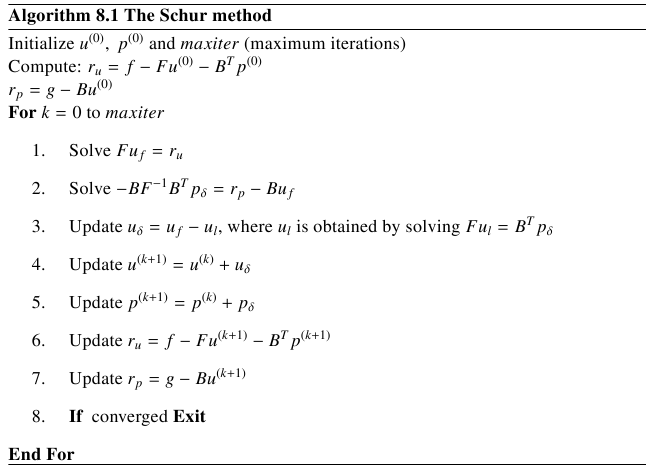
\includegraphics{./SchurAlg.png}
 % SchurAlg.png: 652x470 pixel, 96dpi, 17.25x12.43 cm, bb=0 0 489 352
\end{center}

In this scheme the pressure subsystem in step 2 can be solved by FGMRES (replace $\bf{B F^{-1} B^{T}}$ with $\bf{(B+C) F^{-1} B^{T}}$ In this case we dont construct $(B+C)F^{-1}B^{T}$ but approximately solve $(B+C)F^{-1}B^{T}p_{\delta} = r_{p} -Bu_{f}$. We dont have a good preconditioner for this step but could use something like diagonal scaling.

\section*{References}

On iterative methods for the incompressible Stokes problem, M. ur Rehman, T. Geenen, C. Vuik, G. Segal, and S.P. MacLachlan, International Journal for Numerical Methods in Fluids, to appear, 2011
\input{./CheckImplementation.tex)
\end{document}
